\chapter{Synthesis and Outlook}
\label{cha:out}

\Authors{Olaf Kolditz, Uwe-Jens G\"orke, Heinz Konietzky, Jobst Ma{\ss}mann, Mathias Nest, Holger Steeb, Frank Wuttke, Thomas Nagel}

\section{Synthesis - Directions}

As a result of the GeomInt research project (Chapter \ref{cha:geomint}) a broad combined experimental and numerical platform for the investigation of discontinuities due to swelling and shrinking processes (WP1, section \ref{sec:lab-wp1}), pressure-driven percolation (WP2, section \ref{sec:lab-wp2}) and stress redistribution (WP3, section \ref{sec:lab-wp3}) for important reservoir and barrier rocks (clay, salt, crystalline) has been developed. Model comparisons for damage and fracture processes driven by different processes provide information on the optimal areas of application of the numerical methods (section \ref{sec:synthesis-num}). 

\begin{wrapfigure}{l}{6cm}
\centering
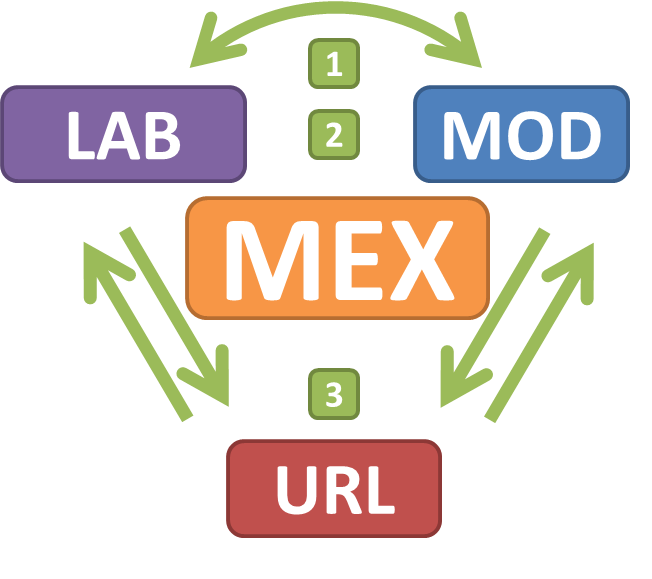
\includegraphics[width=5.9cm]{figures/geomint-mex.png}
\caption{Central MEX concept}
\label{fig:synthesis-mex}
\end{wrapfigure}
A comprehensive validation of the platforms (\glqq{}Proof-of-Concept\grqq) was carried out by ''Model-Experiment-Exercises'' experiments (MEX) for the damage and fracture processes driven by different processes such as swelling and shrinking, pressure-driven percolation and stress redistribution (see chapter \ref{cha:mex}).
The MEX concept is the central synthesis element of GeomInt as it is directly linking models (MOD) with lab experiments (LAB) and paving the way towards the analysis of in-situ experiments (URL) which has been started in the current project phase and will be continued in future activities though (Fig. \ref{fig:synthesis-mex}, see also section \ref{sec:poc}).

The project results allow an improved understanding of the processes, the methods used and the application-oriented systems for realistic time and length scales in order to make the planning and implementation of geotechnical uses of the underground safer, more reliable and efficient. An important part of future work is the transferability of the experimental-numerical concepts and methods to other geotechnological applications (e.g. deep geothermal energy, energy storage, repository problems, methods for hydraulic stimulation, conventional and unconventional resource extraction or tunnel construction). Ongoing activities also aimed to intensify the internationalization started in the previous project in cooperation with complementary research projects (e.g. EURAD, DECOVALEX 2023, Mt. Terri project).
%
In future directions - the basic idea concerning the investigation of the three relevant process types for the formation of pathways in different rock types -- shall be preserved. The proven project structure (WP1-3) is also to be retained (Fig. \ref{fig:geomint2}).

\subsection{Numerical Methods Competencies}
\label{sec:synthesis-num}

Significant emphasis in GeomInt was directed on the development of numerical methods for modelling of discontinuities in various rock types as well as the analysis of advantages / disadvantages of particular methods for specific fracture pattern at various scales (Fig. \ref{fig:num-overview}). The numerical methods have been described in detail in Chapter \ref{cha:num}. The ''competencies'' of the numerical methods under use will be compactly summarized in the following set of tables.

Tab. \ref{tab:num-comp} provides an overview of the capabilities of the numerical methods for simulation of fracturing processes, i.e. (i) crack representation by elements explicitly/separative or by damage variables, (ii) failure criteria, (iii) used mesh types and (iv) fracture aperture calculation.

%Table
\begin{table}[h!]
\centering
\caption{Numerical methods comparison}
\label{tab:num-comp}
\footnotesize
\begin{tabular}{lllll}
\hline
%\rowcolor{cyan}
Methods & Crack representation & Failure criteria   & Mesh & Fracture aperture \\
\hline
LEM     & Element separation   & Element strength   & Lattice        & Direct \\
DEM     & Element separation   & Element strength   & Discrete       & Direct \\
SPH     & Particle based       & NA                 & NA             & Particle based \\
FEM-LIE & Element explicit     & Cohesive law       & Conforming     & Direct \\
FEM-VPF & Damage variable      & Fracture mechanics & Non-conf.      & Indirect \\
FEM-NLD & Damage variable      & Stress based       & Non-conf.      & Indirect \\
FEM-HDF & Element explicit     & Cohesive law       & Conforming and non-conf.  & Direct  \\
\hline
\end{tabular}
\end{table}
\vspace{-5mm}
\tiny Legende: NA - not applicable
\normalsize

The second Tab. \ref{tab:hm-processes} recalls fracturing processes within the adjacent rock mass (i.e. fractured porous medium) for the various rock types (brittle/ductile) investigated in the related work packages (WPs). In the context of hydro-mechanical (HM) coupled processes fluid migration from the fracture into the rock matrix (and vice versa) must be considered for both pre-defined and undefined cracks.

\clearpage

%Table
\begin{table}[h!]
\centering
\caption{Hydro-Mechanics (fracture mechanics) processes}
\label{tab:hm-processes}
\footnotesize
\begin{tabular}{llllll}
\hline
%\rowcolor{cyan}
Rock type         & Crack PD & Crack UD & Leak-off & Non-brittle & Visc. diss.\\
\hline
Clay (WP1)        & yes & yes & maybe & yes & yes \\
Salt/Clay (WP2)   & yes & yes & yes   & yes & yes \\
Crystalline (WP3) & yes & yes & maybe & no  & maybe \\
\hline
\end{tabular}
\end{table}
\vspace{-5mm}
\tiny Legende: PD - pre-defined, UD - undefined, Visc. - viscous, diss. - dissipation
\normalsize

Finally an evaluation of the competencies of all used methods is provided in Tab. \ref{tab:competencies} based mainly on the results of the MEX studies.
An important part of the MEX concept was the application of multiple (at least) methods to these exercises (e.g. for MEX 0-1A three methods, LEM, DEM and FEM-VPF have been applied). For the analysis of lab scale experiments all present methods (discontinuous and continuous) could be applied successfully. The advantages of the discontinuous methods (LEM, DEM) lies in the simulation of small scale processes, e.g. fracture initiation and propagation, and because they rely on the fundamental fracture mechanical phenomena. Discontinuous methods exhibit some difficulties when it comes to coupled processes and at larger scales where continuum methods (FEM\#) are rather strong. We also added 3D capabilities and HPC implementation status to the table.

\newcommand{\done}{\textcolor{green}{\checkmark}}
\newcommand{\perh}{\textcolor{orange}{\checkmark}}
\newcommand{\none}{\textcolor{red}{$\times$}}
%Table
\begin{table}[h!]
\centering
\caption{Methods competencies}
\label{tab:competencies}
\footnotesize
\begin{tabular}{llllllll}
\hline
%\rowcolor{cyan}
Method  & Crack PD & Crack UD & Leak-off & Non-brittle & Visc. diss. & 3D & HPC \\
\hline
LEM     & \done & \done & \done & \done & \done & \done & \perh \\
DEM     & \done & \done & \perh & \done & \done & \perh & \done \\
SPH     & \done & \perh & \done & \perh & \done & \done & \done \\
FEM-LIE & \done & \none & \done & \done & \perh & \none & \none \\
FEM-VPF & \done & \done & \done & \done & \perh & \done & \done \\
FEM-NLD & \done & \done & \perh & \done & \perh & \none & \done \\
FEM-HDF & \done & \none & \done & \perh & \done & \done & \perh \\
\hline
\end{tabular}
\end{table}
\vspace{-5mm}
\tiny Legende: PD - pre-defined, UD - undefined, Visc. - viscous, diss. - dissipation, 3D - three-dimensional simulation, HPC - High-Performance-Computing 
\normalsize

\bigskip
The application of a specific numerical methods is driven by the specific purpose:
\begin{list}{-}{\leftmargin=1em \itemindent=0em \itemsep=0em}
\item fracturing process details, i.e. initiation and propagation
\item process coupling, i.e. THMC
\item scale of application
\end{list}

An important result of GeomInt is the significant further development of individual methods and their extension of application areas \cite{Sattarietal2019b,schmidt2019,Yoshioka2020}, respectively. Therefore, the GeomInt numerical platform as a whole advanced significantly.

\clearpage

\subsection{Proof-of-Concepts}
\label{sec:poc}

Even though the focus of GeomInt was directed on further improvement of modeling and experimental methods, numerical simulation of real-world geotechnical applications is sort of standard meanwhile.
The Proof-of-Concept (PoC) for modelling consists of multiple steps (calibration, validation, verification). Without doubt calibrated models can be provided for individual, site-specific applications - also thanks to the increasing computational power available. The challenge is still, can we reliably transfer models over multiple scales or for various rock types. The latter challenge is subject to GeomInt.

\begin{wrapfigure}{l}{0.5\textwidth}
\vspace{-4mm}
\centering
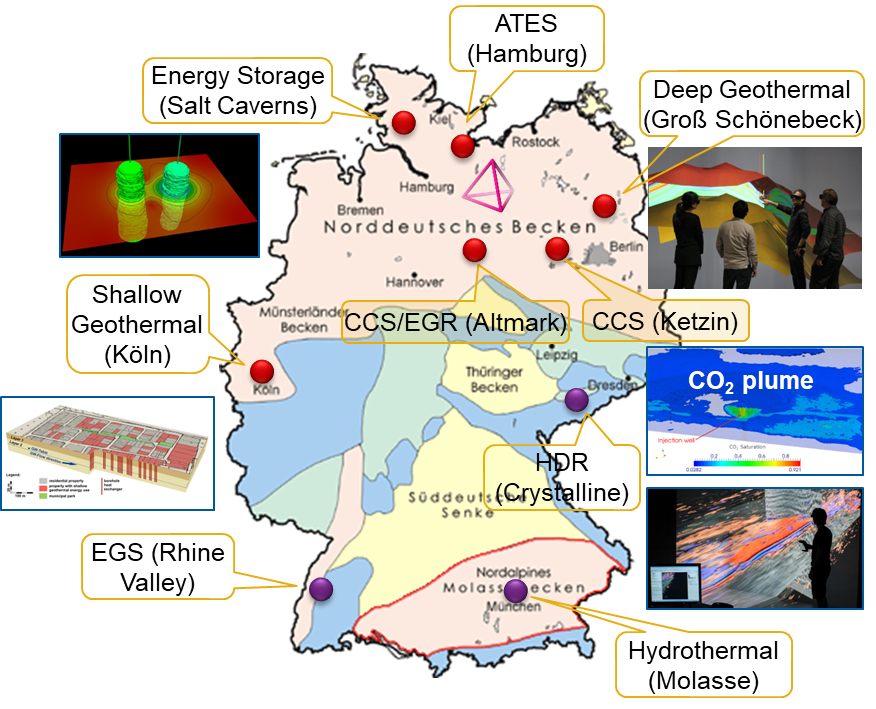
\includegraphics[width=0.49\textwidth]{figures/geoenergy-map}
\caption{OGS applications in the North German Basin}
\label{fig:ogs-ngb}
\end{wrapfigure}
Fig. \ref{fig:ogs-ngb} depicts a number of geotechnical applications in the North-German-Basin (NGB) including shallow and deep geothermal systems, energy storage in aquifers and caverns as well as geological sequestration of carbon dioxide in the subsurface.
All applications studies have been conducted with the OpenGeoSys platform using various T-H-M-C coupled models, i.e. using weak or strong coupling of related thermo-hydro-mechanical-chemical processes. This comprehensive numerical modeling of various geoenergy applications in the NGB may serve as a validation of the THMC concept.

\begin{wrapfigure}{r}{0.5\textwidth}
\vspace{-5mm}
\centering
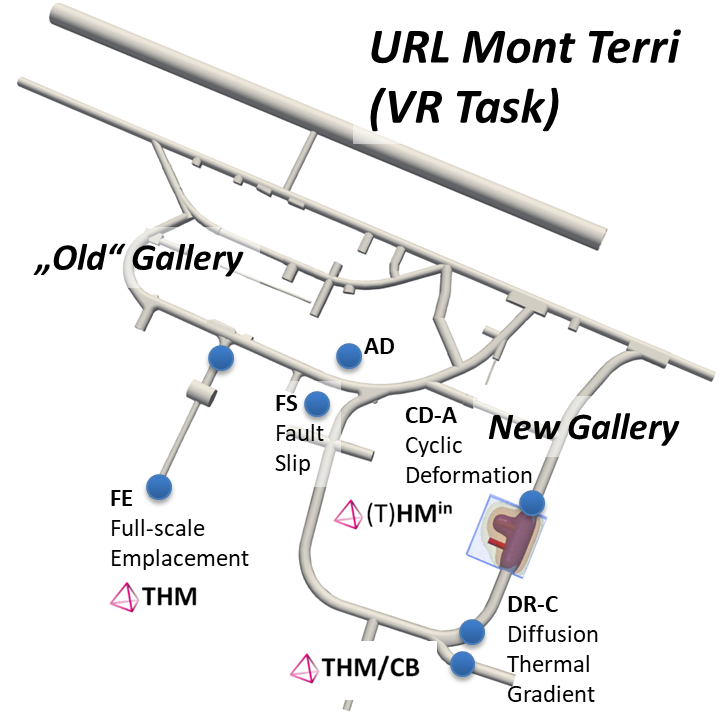
\includegraphics[width=0.49\textwidth]{figures/mt-vr-01a}
\caption{Numerical simulation of various MT experiments \cite{Rink20143857}}
\label{fig:mt-terri}
\end{wrapfigure}
The second Proof-of-Concept study is related to the Underground Research Laboratory (URL) in Mt. Terri where numerous (MT) experiments are conducted simultaneously \cite{Bossart2017405,Bossart20173}. Fig. \ref{fig:mt-terri} shows the tunnels system of the extended URL and a number of ongoing and planned experiments. Numerical simulation is used for both analysis of experimental results and design of new experiments, i.e. for their opti- mal planning. Again OGS is used for the indicated experiments and therefore providing a unified context for numerical simulation. Moreover, all models are included into a Virtual Reality context (see next section).

\subsection*{Information Technology - Digitization}

\begin{wrapfigure}{l}{0.5\textwidth}
\vspace{-3mm}
\centering
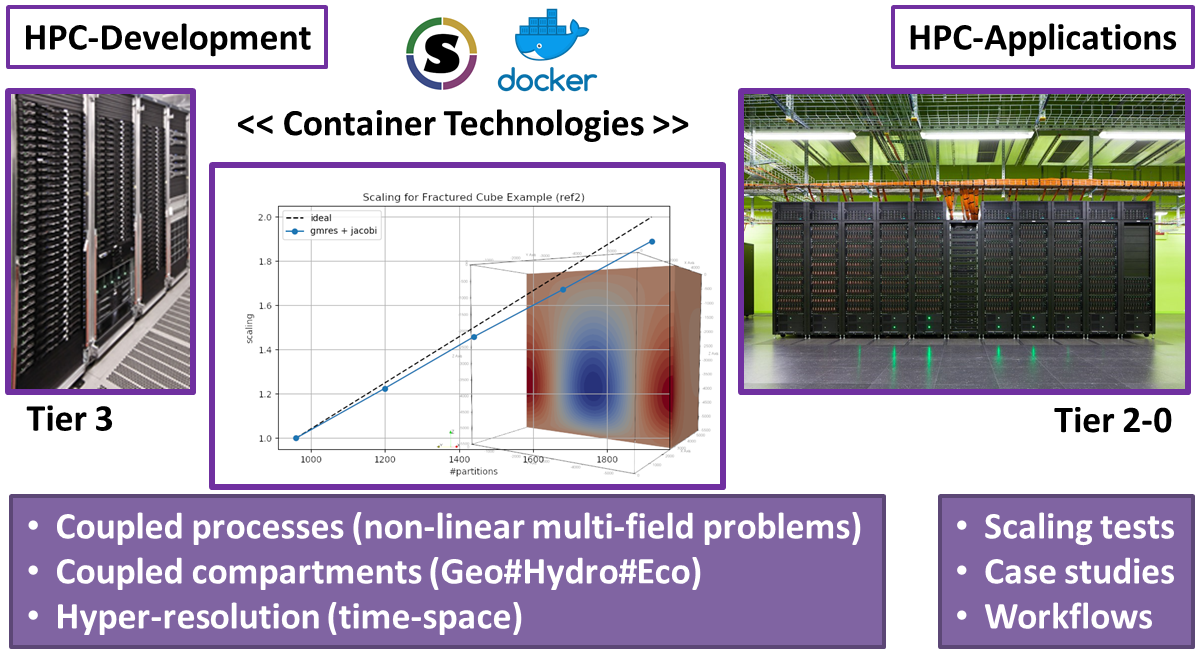
\includegraphics[width=0.49\textwidth]{figures/hpc-concept1}
\caption{High-Performance-Computing}
\label{fig:syn-hpc}
\end{wrapfigure}
Many research areas largely benefit from new developments in information technology in many ways in particular data- and computational geosciences.
Fig. \ref{fig:syn-hpc} shows the HPC concept starting with development and testing methods at smaller machines (Tier 3) and then implementation of high-end infrastructure (Tier 2-0). Container technologies (e.g. Docker, Singularity) are used for standardisation and portability of HPC solutions \cite{Bilke2019}. Scalability of numerical methods for coupled THMC simulations is a particular challenge.

\begin{wrapfigure}{r}{0.5\textwidth}
\vspace{-0mm}
\centering
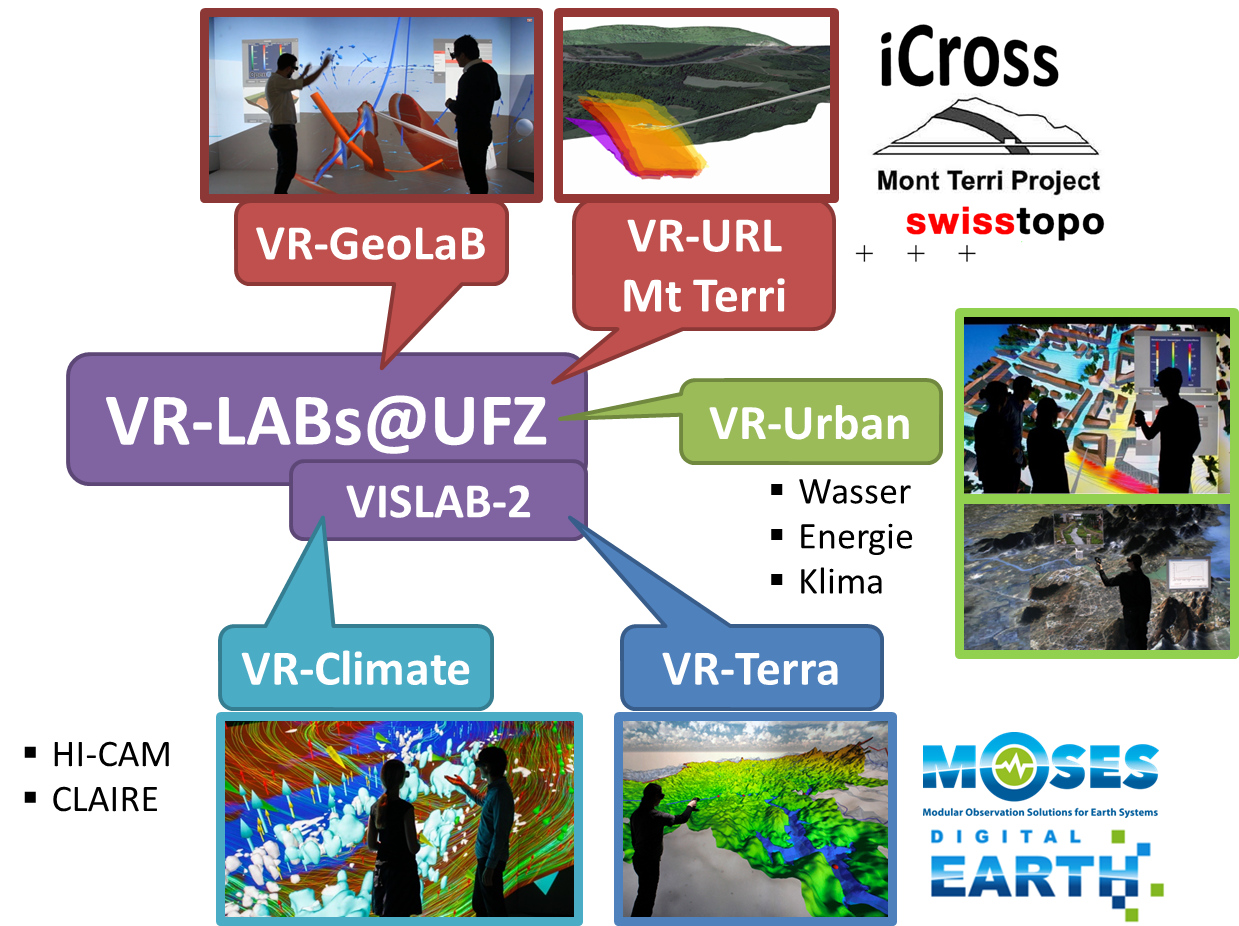
\includegraphics[width=0.49\textwidth]{figures/vr-labs}
\caption{Virtual Reality Labs}
\label{fig:syn-vis}
\end{wrapfigure}
In addition to computational efficiency, visual data analysis is promising field for many domain sciences as well. Fig. \ref{fig:syn-vis} depicts several examples of visualisation from environmental sciences concerning terrestrial (hydrology), atmospheric (climate research), and geological systems. Virtual Reality concepts allow for the combination of various kind of data and models in a real geo-referenced context - making those integrated VR Labs a useful planning tool e.g. for experimental design in URLs or infrastructures for urban systems.

\begin{wrapfigure}{l}{0.5\textwidth}
\vspace{-3mm}
\centering
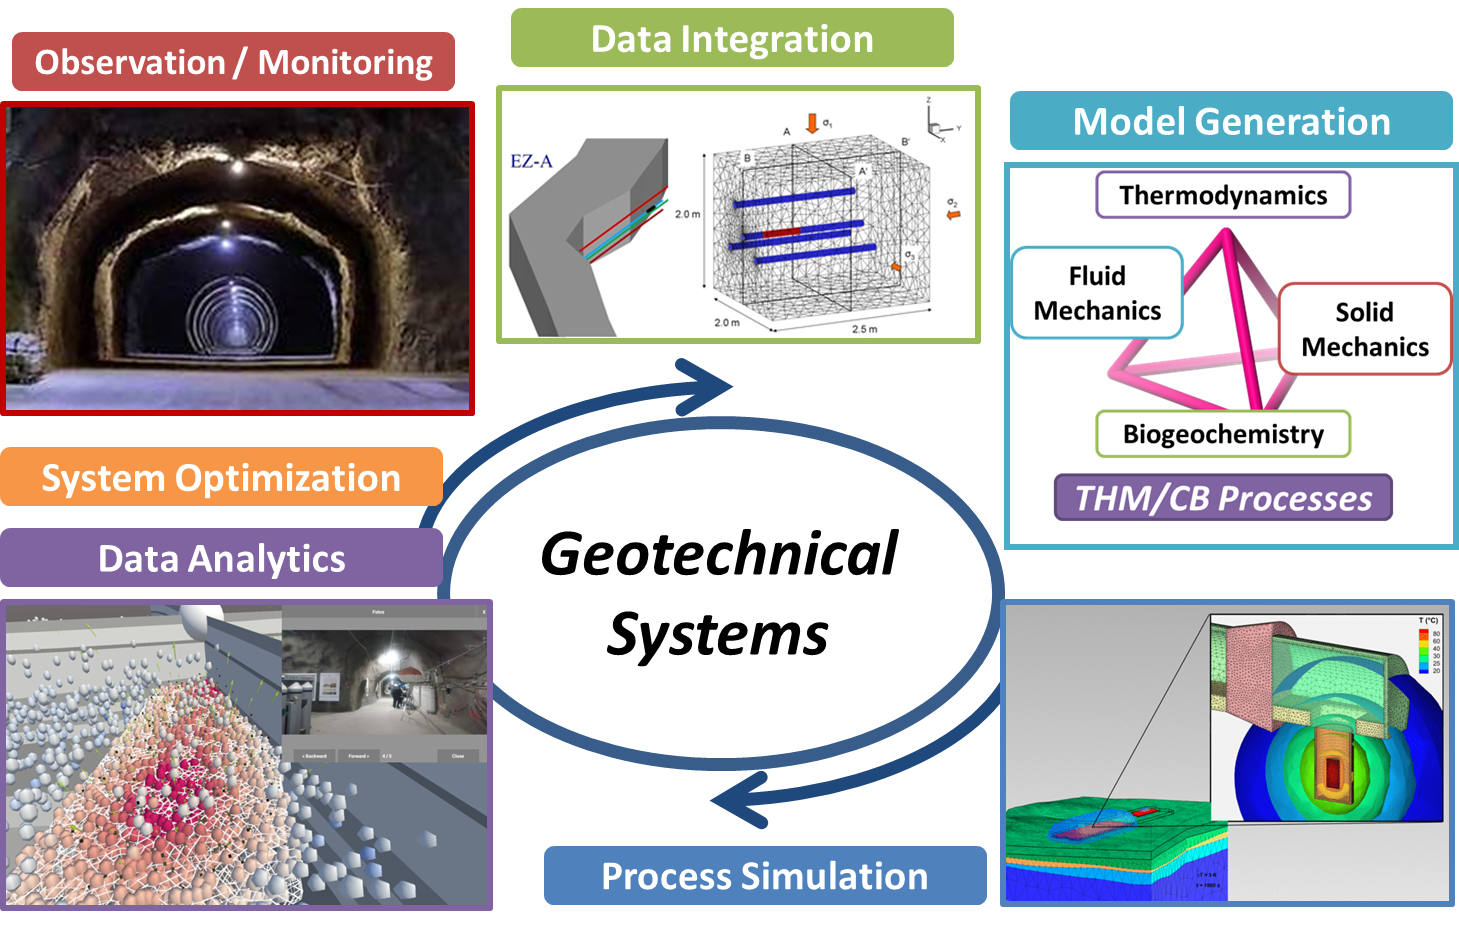
\includegraphics[width=0.49\textwidth]{figures/workflow-geotechnics}
\caption{Seamless analysis Workflows}
\label{fig:syn-workflows}
\end{wrapfigure}
Intelligent use of Information Technology will foster the development and implementation of seamless analysis workflows in many research areas. Fig. \ref{fig:syn-workflows} illustrates the concept for geotechnical applications starting with data integration from URLs, set-up of adequate models for experimental analysis and design. HPC concepts for THMC simulations allow realistic analysis of process complexity and predictions. Virtual Reality makes outcomes accessible for specialists and a public audience as well.

\clearpage

\subsection{International Collaboration}

\begin{wrapfigure}{r}{0.25\textwidth}
\vspace{-5mm}
\centering
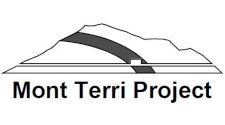
\includegraphics[width=0.24\textwidth]{figures/mont-terri}
%\caption{}
\label{fig:workflows}
\end{wrapfigure}
GeomInt benefited to a huge extend from international cooperation and produced an impact vice versa. Clay samples of both the shaly an sandy facies from the URL Mt. Terri were the basis for experimental work with Opalinus clay. GeomInt models for variuos MT experiments embedded into a VR context helped the ''Proof-of-Concept'' for experimental analysis and design of future campaigns.

\begin{wrapfigure}{l}{0.25\textwidth}
\vspace{-1mm}
\centering

\includegraphics[width=0.24\textwidth]{figures/decovalex-2019}
%\caption{}
\label{fig:workflows}
\end{wrapfigure}
GeomInt's MEX concept is mainly derived from the DECOVALEX benchmarking tasks idea by closely combining own experimental with modelling works. Using different (continuous and discontinuous) numerical methods helped the general process understanding and elaboration of particular methods' dis-/advantages as well. GeomInt partners will participate the new DECOVALEX 2023 phase. 

\begin{wrapfigure}{r}{0.25\textwidth}
\vspace{-5mm}
\centering
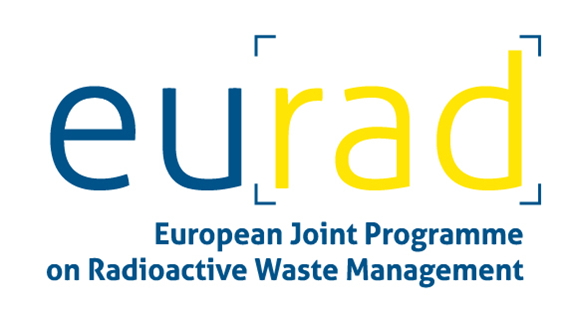
\includegraphics[width=0.24\textwidth]{figures/eurad}
%\caption{}
\label{fig:workflows}
\end{wrapfigure}
GeomInt's concept and project results will be deployed for the new European Joint Program on Radioactive Waste Management EURAD. In addition to Opalinus clay (OPA), EURAD is dealing with various European clays such as Callodo-Oxfordian (COx) and Boom clay and providing a European knowledge base for clays as barrier rock for waste isolation and energy storage.

\subsection*{Webpage}

The webpage of GeomInt (Fig. \ref{fig:geomint-web}) is the entry point an reference of the project. It contains an overview of the project as well as quarterly updated news of ongoing activities. GeomInt publications are listed and an access point to the data management system is provided (see Chapter \ref{cha:dms}).

\begin{figure}[ht!]
\centering
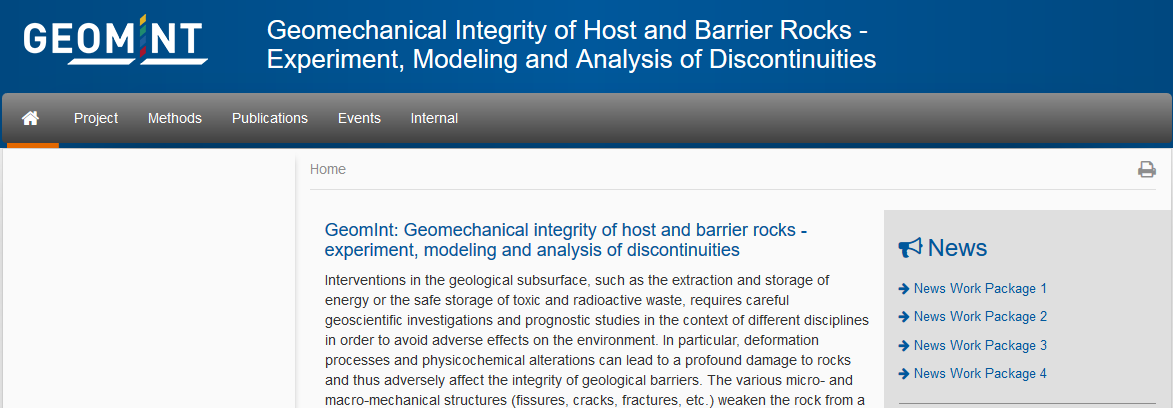
\includegraphics[width=0.95\textwidth]{figures/geomint-web.png}
\caption{Webpage of the GeomInt project $\Rightarrow$ \url{www.ufz.de/geomint}}
\label{fig:geomint-web}
\end{figure}

\begin{figure}[ht!]
\centering
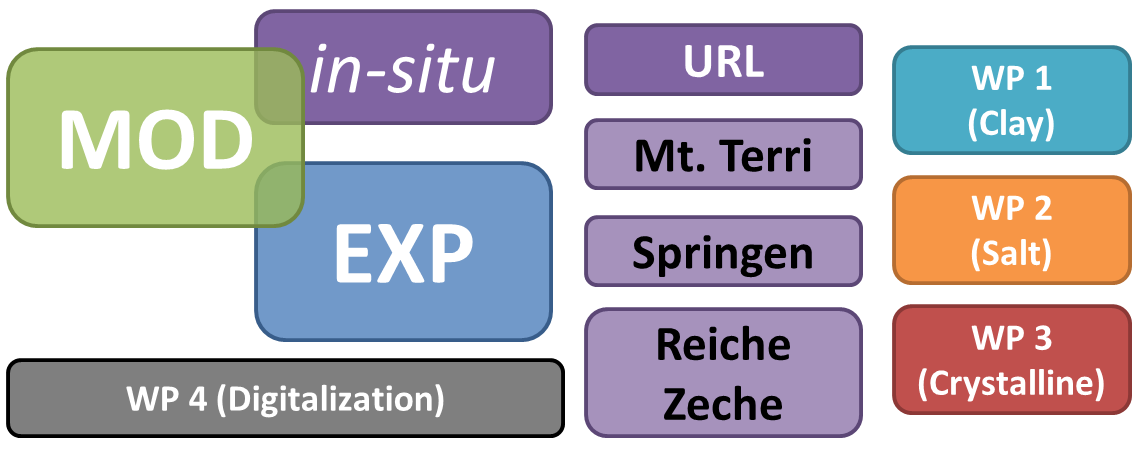
\includegraphics[width=0.85\textwidth]{figures/geomint2.png}
\caption{Graphical abstract of the GeomInt research concept}
\label{fig:geomint2}
\end{figure}

\section{GeomInt Outlook - Future Work}

After a very strongly methodically oriented first phase, the continuation project is intended to demonstrate practical applicability under real conditions (URLs). Furthermore, knowledge gaps in the experimental as well as numerical field shall be closed.

GeomInt is to be worked on by the interdisciplinary consortium of partners from universities, public and private research institutions with complementary, long-standing experience in the analysis of geosystems, which has proven itself from the previous project. New findings are expected, in particular regarding system understanding of the effects of discontinuities on underground geosystems. In this context, the focus of experimental investigations will shift significantly to the performance and evaluation of in-situ experiments in various underground laboratories (URLs). For the efficient numerical simulation of coupled mechanical, thermal and hydraulic processes in the formation and development of discontinuities on the scale under consideration, the adaptation of models and algorithms investigated and further developed in GeomInt to methods of high-performance computing (HPC) is a new aspect. The descriptive presentation of structural, experimental and model results in the real context (e.g. URLs) is to be carried out within the framework of an integrated visual data analysis (virtualization).
In the figure \ref{fig:geomint2} shows a graphical illustration of the project continuation.

Future research will contain following aspects:
\begin{list}{--}{\leftmargin=1em \itemindent=0em \itemsep=-0.5em}
\item experiments: The focus is on the evaluation of the latest in-situ experiments in the rock\-laboratories Mt. Terri (Opalinus clay), Springen (salt) and Reiche Zeche (crystalline). Selected laboratory experiments are planned in order to specifically close still existing knowledge gaps (e.g. mechanical anisotropy of clay rocks).
\item modelling: Numerical methods are to be further developed and applied for in-situ use in a focused manner. For the scaling from micro- to macroscale models, different model approaches are to be specifically linked together (e.g. integration of the LEM in the FE method).
\item digitization: New developments in computer science, such as high-performance computing and visual data analysis, will be incorporated into the continuation of the project. This is necessary on the one hand to achieve the necessary scaling of the models (from micro to macro scale) and on the other hand to allow the representation of the model results in the real context of the underground laboratories.
\item Internationalization: In addition, international cooperation with the Mt. Terri project and DECOVALEX 2023 will be intensified, also to increase the visibility of the Geo:N project.
\end{list}

\section{Pathways through swelling and shrinking processes}
\label{sec:wp1-plan}

\begin{wrapfigure}{l}{0.5\textwidth}
\vspace{-5mm}
\centering
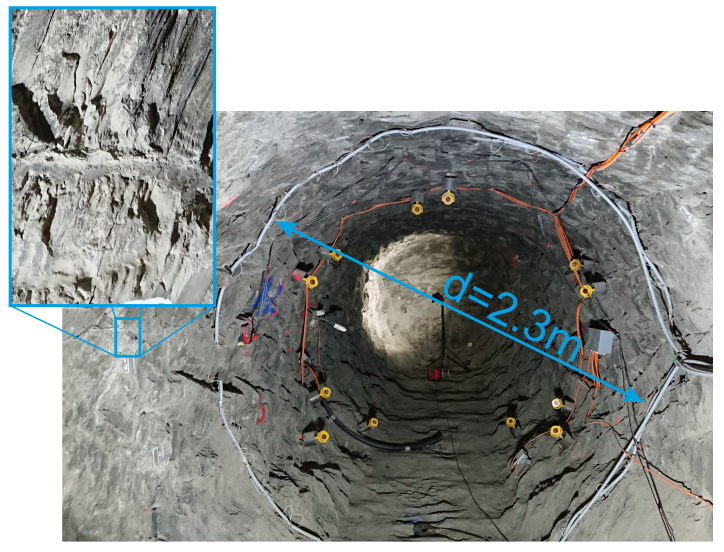
\includegraphics[width=0.49\textwidth]{figures/CDA_open_niche}
\caption{URL Mt. Terri: CD-A experiment: desaturation cracks at the ventilated open niche (Photo: BGR)}
\label{fig:cd-a}
\end{wrapfigure}
The focus of the work in the continuation is the Mt. Terri CD-A experiment. In autumn 2019, two 11\,m long niches were excavated and extensively instrumented. While one niche is ventilated and thus exposed to seasonal fluctuations in humidity, the second niche is kept closed by a bulkhead. First geophysical measurements as well as observations of drying cracks on the walls already indicate the influence of desaturation in the ventilated niche, while the closed niche, where a constantly high humidity has been established, does not show any such cracks. Based on the experimental analyses, the anisotropic swelling and shrinking behaviour under these boundary conditions is analysed and characterised in the laboratory. The analysis is the basis for further modelling on larger scales. 
The numerical methods \cite{Yoshioka2019,Parisio2019102} developed in GeomInt are to be used and, if necessary, further refined in order to model and analyse the observed differences between the two niches. In a first step, the two-dimensional HM calculations of the CD/LP experiment (in \cite{Kolditz2020b}) performed within GeomInt will be extended by the newly developed non-linear transversal-isotropic approaches in mechanics and in the swelling and shrinking model. Furthermore, the possibility of modelling shrinkage cracks in the HM context is investigated on the mechanical side by the phase field method and plastic models and on the hydraulic side with multicontinua models. In a second step, this approach will be applied to the CD-A experiment and quantitatively analyzed by comparison with measured data, so that a basic validation of the model approach on field scale is possible. 

\section{Displacements due to pressure-driven percolation}

\subsection{Pressure-driven percolation in clay rock under in-situ conditions}

\begin{wrapfigure}{l}{0.5\textwidth}
\vspace{-5mm}
\centering
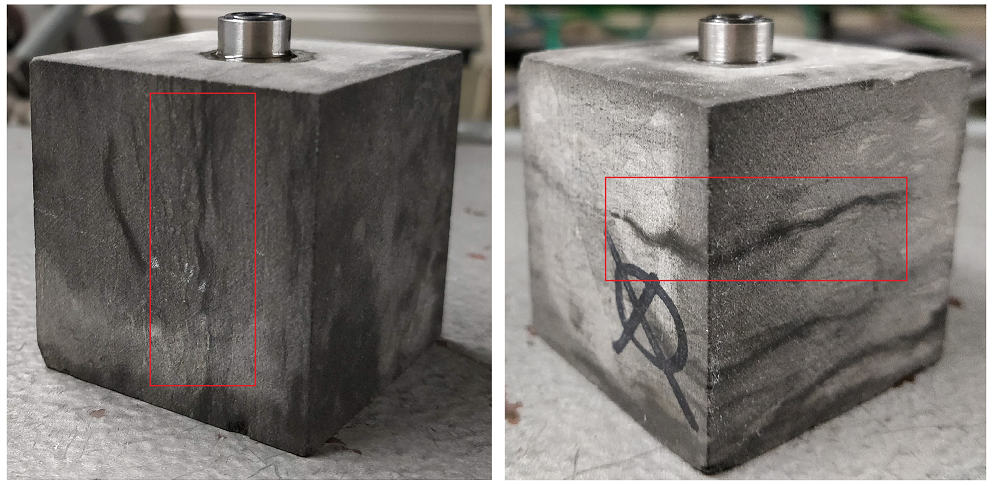
\includegraphics[width=0.49\textwidth]{figures/GeomInt_AP2_CAU}
\caption{Pathways through pressure-driven percolation, clay rock (Photo: CAU Kiel)}
\label{fig:cd-a}
\end{wrapfigure}
In the GeomInt continuation, the laboratory-experimental focus is on the investigation of anisotropy effects. This material state determines all physical properties, especially for claystone. For the characterization of the anisotropic material behavior, in particular fracture behavior and pathability under temperature, saturation and pressure changes are to be analyzed. Selected investigations, e.g. fracture toughness analyses, fluid-driven percolation tests or high-pressure cube pressure tests are to be carried out with special consideration of the material anisotropy. Any additional material samples that may be required could be provided by ongoing drilling activities in the new galleries in the Mt. Terri rock laboratory. The aim is to determine the anisotropic fracture and strength parameters, conductivities or fracture paths required for further simulations during fluid percolation under in-situ conditions.

The already developed thermo-hydro-break-mechanical lattice element method (LEM) is used with a vectorized meshing for anisotropic boundary conditions and verified by the above mentioned specific laboratory tests. 
%
For the transition from micro- or mesoscale LEM to macroscale FEM simulations, the \glqq Mesh Fragmentation Technique (MFT)\grqq{} is to be extended in such a way that vectorized Voronoi LEM grids are directly transferred to the finite element meshes according to the MFT. The material properties of the MFT interface elements are then replaced by the physical fracture properties of the lattice beams. Since a pre-definition of the crack path is not necessary with this approach even in large scale FE models, this approach is extremely attractive for future realistic simulations.
%
The planned combination of LEM with FEM and thus a consideration of micro-properties for larger scale simulations corresponds to the concept of the GeomInt continuation regarding scaling from laboratory to in-situ scale and thus the direct use of the GeomInt2 modeling platform for URL experiments.

The LIE method \cite{Vowinckel2020}, which has been further developed in GeomInt, will also be used to simulate pressure-driven crevice reactivation in another Mt. Terri experiment (Fault-Slip FS experiment). The hydromechanical coupling is investigated in the case of an inelastic change in the properties of an existing fissure or crack network in the claystone as a result of fluid injection. Due to the special boundary conditions, modeling is of particular importance for the interpretation of this complex in-situ experiment, since the observed behavior in laboratory experiments can only be simulated in a very simplified way.

\subsection{Pressure-driven percolation in salt rock under in-situ conditions}

\begin{wrapfigure}{l}{0.5\textwidth}
\vspace{-5mm}
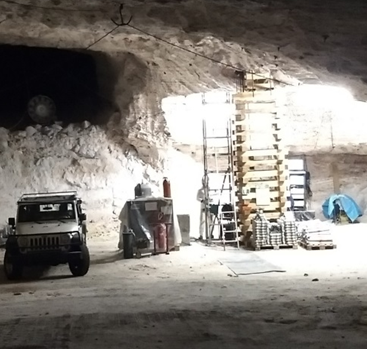
\includegraphics[width=0.49\textwidth]{figures/Versuch-Photo.png}
\caption{Underground laboratory Springen}
\end{wrapfigure}
In the in-situ laboratory of the Springen mine, a large bore hole of 50\,m$^3$ is used to investigate the pressure-driven percolation of both liquids and gases. This was carried out with compressed air, representative of natural gas, and the rupture of the rock was monitored by an array of sensors for acoustic emissions. This large-scale experiment will be evaluated in two ways in the continuation. On the one hand, the influence of the local stress field and the rupture zone on pressure development and propagation direction shall be investigated by means of a discontinuum mechanical method. On the other hand, it shall be determined whether the same process can be reproduced with a continuum mechanical method. The model application is again driven by the idea of scaling from the smaller to the larger in-situ scale.
As an extended continuum mechanical approach, the phase field method is used to simulate the large-scale Springen experiment. 
%
It is planned to compare the two methods (FLAC3D and OpenGeoSys phase field method) with regard to their suitability for scalability to larger systems. This will also involve computational efficiency using HPC methods (parallelisation).

\section{Displacements due to stress redistribution}

In the continuation of the project, there is the chance to observe on a smaller scale selected phenomena of the hydro-mechanically coupled behaviour of discontinuities, which were integrally investigated in the previous work package, i.e. averaged over the size of the sample on the cm to dm scale. For this purpose, test paths for mechanical and hydraulic scenarios can be built up on the experimental basis already developed with regard to the boundary conditions. 
In particular, the discretization of the shear surfaces with the aid of the 3D scanner represents the link between the measured hydro-mechanically coupled fracture behaviour and local phenomena in the mm range. 
%
Methodologically, a further development towards observational procedures, which allow an appropriate spatial resolution (at least in the mm range) with simultaneous mechanical or coupled loading of the fissure body sample, is being carried out. Specifically, the shear box of the shear apparatus in the Freiberg laboratory is modified in such a way that the arrangement of piezoceramic sensors for recording acoustic emissions (AE) and the fixing of micro-accelerometers directly next to, or above and below the fissure surface is possible. By operating the AE sensors in active mode, i.e. as ultrasonic actuators for pulse generation, damage parallel to the fissure surface and dislocation on the fissure surface can be quantified. The combined use of the AE system and the microseismic network significantly improves the possibilities for locating the damage processes and for generating the hearth surface solution, since shear waves can now also be reliably detected in their 3D spatial position. In contrast to AE sensors, the micro-accelerometers also provide measurement data on the absolute energy of the recorded seismic events, thus enabling quantitative analysis of the crack initiation process in its spatio-temporal evolution.

The gneiss from Freiberg (URL Reiche Zeche) is selected as sample material, with the focus primarily on fissures and fault zones in the otherwise massive gneiss body. Since preliminary tests showed that the foliation of the gneiss is mechanically visible but hydraulically only of limited relevance, crevasses and fault zones were identified as potential pathways in the gneiss.
%
The Freiberg data from the experimental tests are directly used by the Stuttgart team for numerical simulation to characterize the hydro-mechanical coupling of fluid-saturated cracks or fracture networks (using hybrid FE methods). Transient stimulation experiments will be simulated. The combination of e.g. harmonic pump experiments and the numerical simulation tools developed here allows a realistic description of the pressure-dependent effective permeability of the crack networks as well as an estimation of the associated effective crack storage capacity.

This research focus will also strengthen the international networking of GeomInt2 with the DECOVALEX 2023 project. There it is planned to work on complementary objectives to the work package described here - for example, on fissure behavior under thermal or polyaxial boundary conditions. 

Both projects GeomInt2 and STIMTEC2 want to strengthen their cooperation in the continuation. Of great interest for GeomInt2 are the experimental stimulation experiments of the STIMTEC project in the rich coal mine \cite{steeb-2020c} for testing the modeling platform under in-situ conditions. For STIMTEC2 the determination of mechanical and hydraulic properties for the crystalline (characterization of fault zones, fractures and rock matrix) from the GeomInt2 concept is of particular interest. Thus both projects can create significant added value in the cooperation.

%Eine internationale Zusammenarbeit ist auch in der Zukunft weiterhin geplant. Hierzu sollen ebenfalls  Stimulationsexperimente im geklüfteten kristallinen Gestein (Grimsel) vertiefend ausgewertet und untersucht werden, vgl. aktuelle Kooperation \cite{steeb-2020b}.

\section[Data and model integration]{Data and model integration using virtualization and high-performance computing}

In the context of the follow-up project, the synthesis activities are to be strengthened. In particular, modern methods of digitization will be further developed and applied. This includes scientific software development, virtualization and high-performance computing - which will be applied specifically to selected GeomInt studies in the sense of demonstrating the GeomInt platform.

\begin{wrapfigure}{l}{0.5\textwidth}
\vspace{-5mm}
\centering
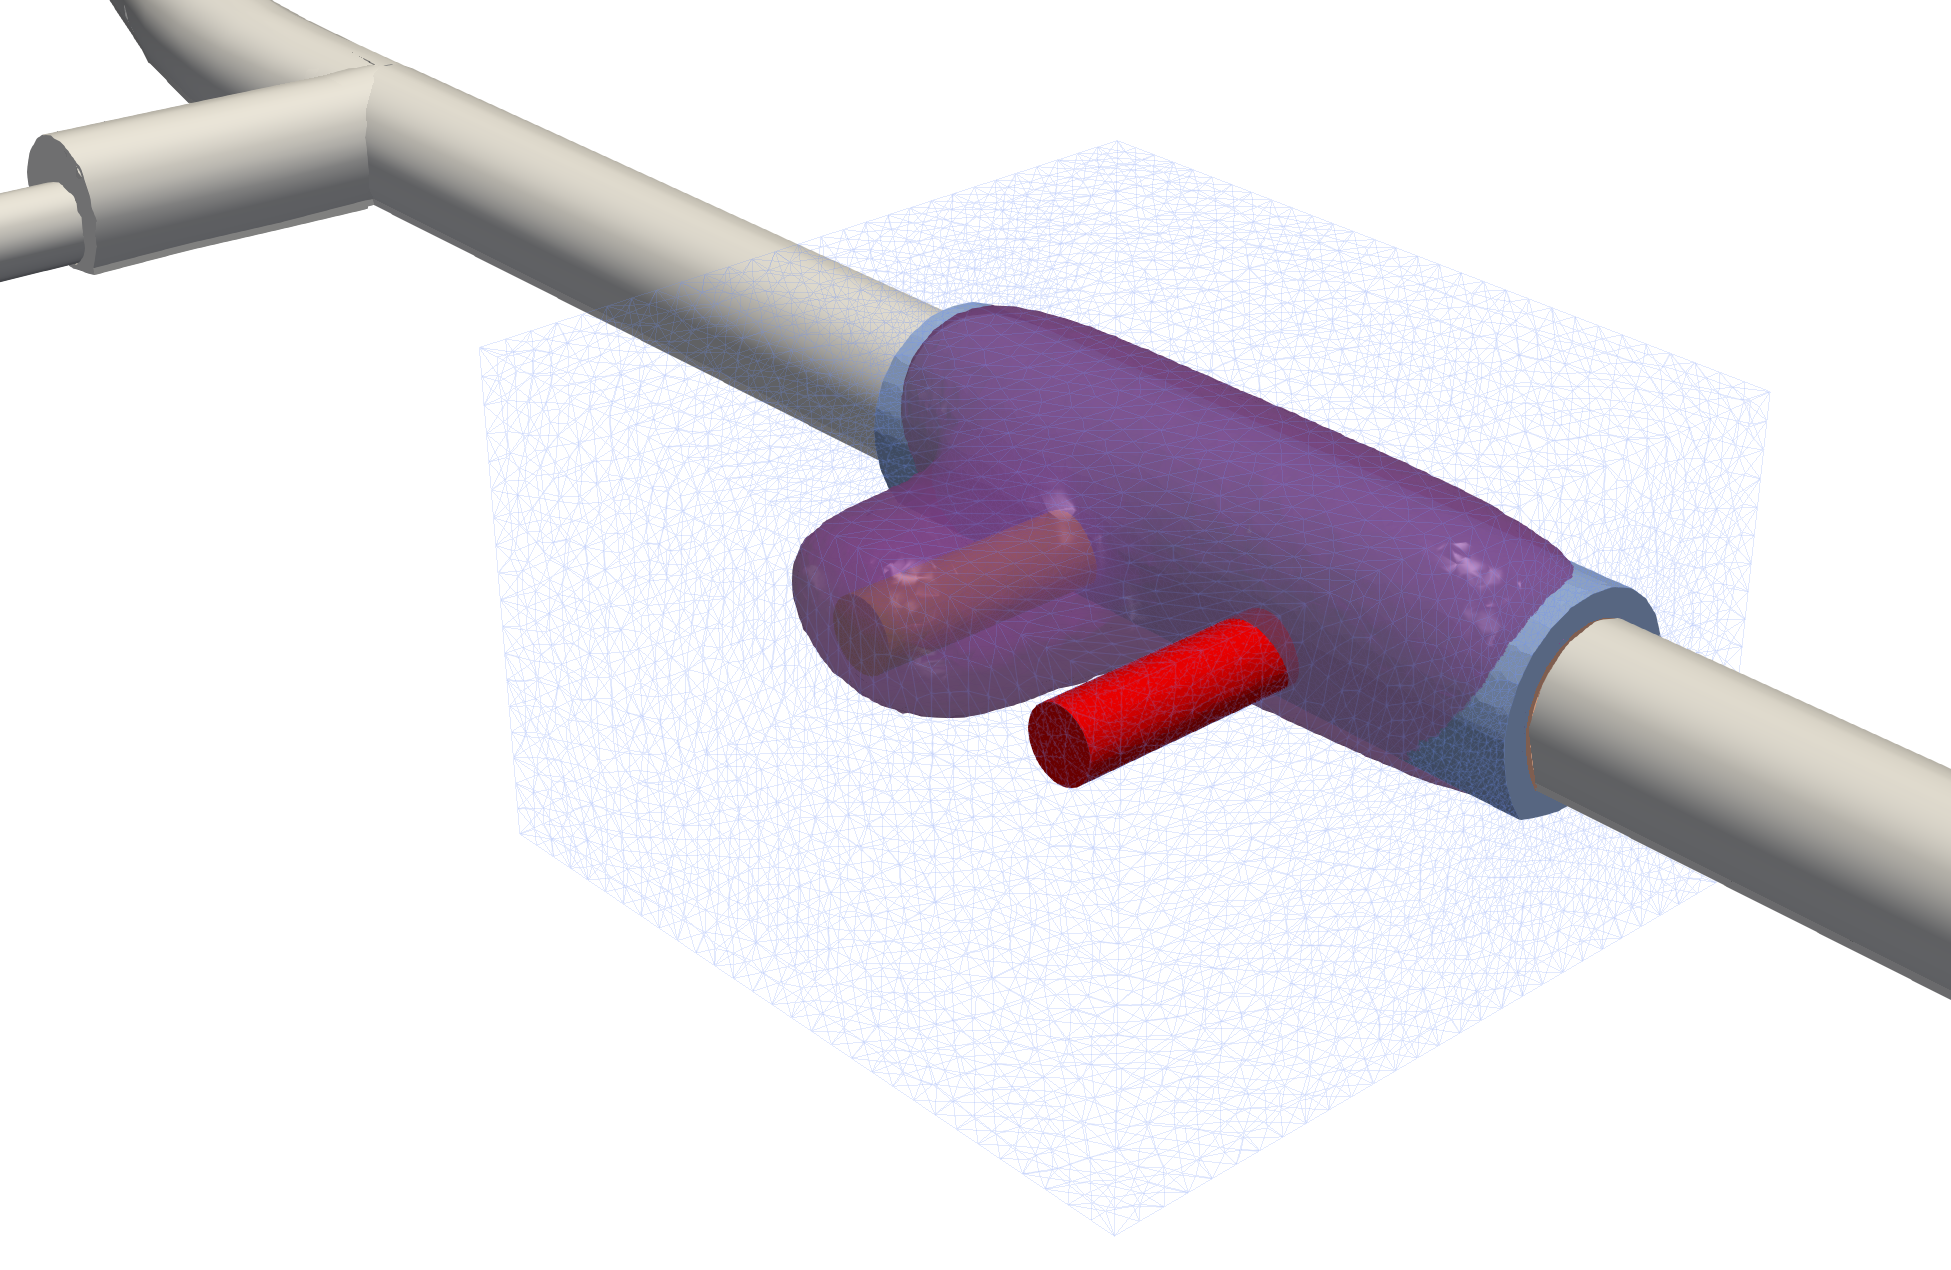
\includegraphics[width=0.49\textwidth]{figures/cd-a}
\caption{Virtualization of the CD-A experiment (Source: BGR/UFZ)}
\label{fig:cd-a}
\end{wrapfigure}
The procedure will be explained using the example of the CD-A experiment in the underground laboratory at Mt. Terri (see section \ref{sec:wp1-plan}). In the first project phase, the constitutive model was developed and implemented \cite{Vowinckel2019}. In order to use the models as realistically as possible, they are built into the underground laboratory using virtualization (see figure \ref{fig:cd-a}). The model has already been used for the planning of the CD-A experiment to determine the optimal distance between the niches (no significant interaction within 20 years). A further increase of the process complexity (nonlinear mechanics in the HM context) requires the unconditional use of HPC methods to simulate a large number of variants. The model results should be continuously compared with the running experiments and also integrated into the existing virtualization context. This is the basic idea of continuous data and model integration.


